\vspace{1em}

\usetikzlibrary{graphs, positioning, quotes, shapes.geometric}

\begin{document}
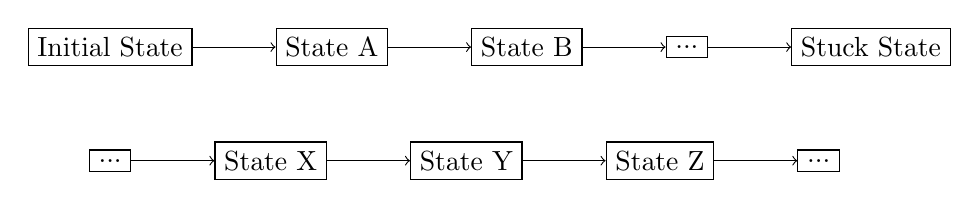
\begin{tikzpicture}[node distance=10pt]
    \node[draw]                           (State 0)  {Initial State};
    \node[draw, right=30pt of State 0]    (State 1)  {State A};
    \node[draw, right=30pt of State 1]    (State 2)  {State B};
    \node[draw, right=30pt of State 2]    (State 3)  {...};
    \node[draw, right=30pt of State 3]    (State 4)  {Stuck State};

    \node[draw, below=30pt of State 0]     (State 5)  {...};
    \node[draw, right=30pt of State 5]     (State 6)  {State X};
    \node[draw, right=30pt of State 6]     (State 7)  {State Y};
    \node[draw, right=30pt of State 7]     (State 8)  {State Z};
    \node[draw, right=30pt of State 8]     (State 9)  {...};
    
    \graph{
        (State 0) -> (State 1) -> (State 2) -> (State 3) -> (State 4);
        (State 5) -> (State 6) -> (State 7) -> (State 8) -> (State 9);
    };
\end{tikzpicture}